\chapter{Knapsack Problem 0/1 - Il Problema dello Zaino 0/1}
Questione da risolvere: trovare il subset di oggetti di massimo valore complessivo
che non superi la capacità C.
\paragraph*{Oggetti} Ad ogni oggetto viene associato un peso e un valore, quindi il problema
consiste nel inserire nello zaino il massimo valore possibile senza superare il peso massimo.
\section{Istanza del problema}
Insieme di n oggetti $\{1,2,\dots,i,\dots,n\}$:
\begin{itemize}
    \item C \ra Capacità dello zaino
    \item $v_n$ \ra Valore dell'oggetto n
    \item $w_n$ \ra peso/ingombro dell'oggetto n
\end{itemize}
\paragraph*{Esempio}
\begin{center}
    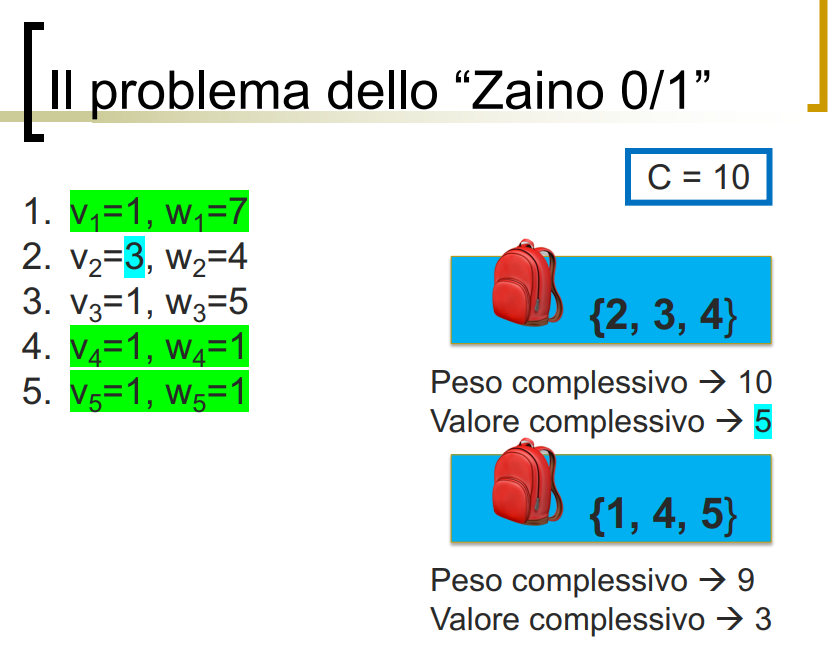
\includegraphics[width=100mm, scale=0.5]{chapters_ulerich/img/knapsack_example.png}
\end{center}
\section{Definizione formale}
Dato un insieme $X=\{1,2,\dots,i,\dots,n\}$ di n oggetti, un intero C e due funzioni:
\begin{itemize}
    \item $V:X \rt N$ tale che $V(i) = v_i$ è il valore dell'oggetto i
    \item $W:X \rt N$ tale che $W(i)=w_i$ è il peso dell'oggetto i
\end{itemize}
si vuole trovare un sottoinsieme $S=\{i_1,i_2,\dots, i_k\}$ di X tale per cui:
\begin{align*}
    W_S=&\sum^k_{j=1}w(i_j) \leq c\\
    V_S=&\sum^k_{j=1}v(i_j)
\end{align*}
Dove $V_S$ è il massimo tra tutti i valori dei possibili sottoinsiemi di X che sono "compatibili" con lo zaino.\\
Si tratta dunque di un problema di ottimizzazione di massimo, dove:
\begin{itemize}
    \item (n,C) \ra dimensione del problema
    \item Soluzioni possibili \ra tutti i sottoinsiemi $S'$ di X il cui peso totale $W_{S'}$ è al più la capacità C
    dello zaino
    \item Funzione obiettivo \ra valore totale $V_{S'}$ della soluzione possibile $S'$.
    \item Valore totale di S \ra valore ottimo
    \item S \ra Soluzione ottimale
\end{itemize}
\subsection{Soluzione del problema DP}
\begin{enumerate}
    \item Calcolo del valore ottimo (valore totale di S)
    \item Ricostruzione di una soluzione ottimale (un insieme S)
\end{enumerate}
\section{Sottostruttura Ottima}
Consideriamo l'esempio di inizio capitolo:
\begin{center}
    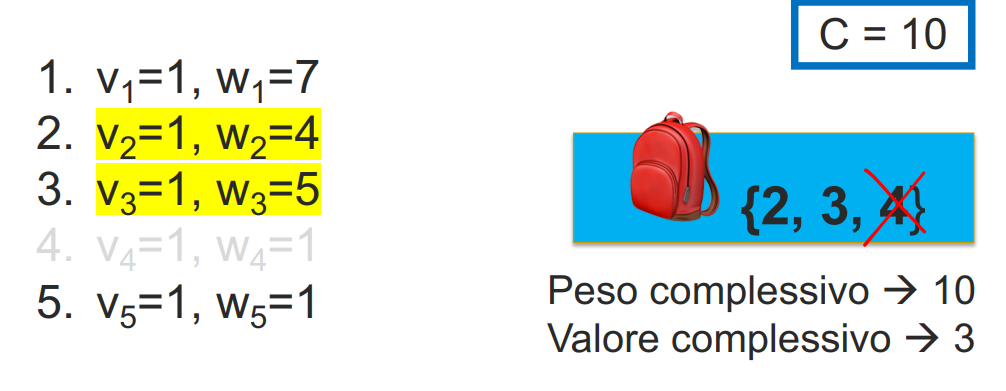
\includegraphics[width=80mm, scale=0.5]{chapters_ulerich/img/knapsack_ricerca_sott_ott.png}
\end{center}
$\{2,3\}$ è una soluzione ottimale di $X \setminus \{4\}$? \textcolor{red}{NO}.\\
$\{2,3, 5\}$ è una soluzione ottimale di $X \setminus \{4\}$!\\
\subsection{Diamo un ordine agli oggetti}
Diamo un ordine agli oggetti all'interno di X, cioè:\\
1 viene prime di 2 che viene prima di 3, etc. che viene prima dell'ultimo oggetto n.\\
\paragraph*{Data una soluzione ottima S si può verificare}
\begin{itemize}
    \item \textbf{CASO 1}: l'oggetto n appartiene a S
    \item \textbf{CASO 2}: l'oggetto n NON appartiene a S
\end{itemize}
\paragraph*{CASO 1} $C \geq w_n$ e l'oggetto n appartiene a S.\\
NB: $S' = S \setminus \{n\}$ non è necessariamente la soluzione ottimale dell'istanza per
$X \setminus \{n\}$ e capacità C.
%Arrivato a Slide 33

